\documentclass[9pt,conference,a4paper]{IEEEtran}
\IEEEoverridecommandlockouts

\usepackage{graphicx}
\usepackage{floatrow}

\title{Constrained spherical deconvolution \\ on signal and ODF values}
\author{
	\IEEEauthorblockN{
		Eleftherios Garyfallidis\IEEEauthorrefmark{1},
		Samuel St-Jean\IEEEauthorrefmark{1},
		Michael Paquette\IEEEauthorrefmark{1},
		Pierrick Coup\'e\IEEEauthorrefmark{2},
		Maxime Descoteaux\IEEEauthorrefmark{1}
	}

	\IEEEauthorblockA{\IEEEauthorrefmark{1} Sherbrooke Connectivity Imaging Lab (SCIL), Computer Science department, Universit\'e de Sherbrooke, Sherbrooke, Canada}
	\IEEEauthorblockA{\IEEEauthorrefmark{2} CNRS, Laboratoire Bordelais de Recherche en Informatique, Bordeaux, France}
}

\begin{document}
\maketitle

For the purpose of the ISBI HARDI reconstruction challenge 2013 and for the categories DTI and HARDI acquisitions, we reconstructed the diffusion datasets using two well established methods: a) Spherical Deconvolution Transform (SDT) \cite{descoteaux-deriche-etal:09}, \cite{Descoteaux2008} and b) Constrained Spherical Deconvolution (CSD) \cite{tournier-calamante-etal:07}.

The SDT is a sharpening operation which transforms the smooth diffusion ODF into a sharper fiber ODF. The method is inspired by CSD \cite{tournier-calamante-etal:07} with, the main difference that the CSD is applied directly to the initial signal and the SDT directly to the ODF. 

The idea here is that an ODF, for example the analytical Q-ball ODF $\psi_{QBI}$, can be formed by the convolution between the single fiber diffusion ODF kernel $R$ and the true fiber ODF $\psi_{SDT}$. 
\begin{equation}
\psi_{QBI}(\mathbf{u})=\displaystyle\int_{|w|=1} R(\mathbf{u} \cdot \mathbf{w}) \psi_{SDT}(\mathbf{w}) dw\label{eq:Conv}
\end{equation}
Therefore, the deconvolution of $\psi_{QBI}$ can recover a sharper $\psi_{SDT}$. We can derive the formula for the $\psi_{SDT}$ using symmetrized spherical harmonics.
\begin{equation}
\psi_{SDT}(\mathbf{u})=\displaystyle\sum_{j=1}^{R}2\pi P_{l_{j}}(0) \frac{c_j}{f_j}Y_{j}(\mathbf{u})\label{eq:ODF_SDT}
\end{equation}
For the derivation and explanation of the formula see \cite{descoteaux-deriche-etal:09}.

The deconvolution that we used here is a fast converging iterative process. Usually, taking 5 to 10 iterations for convergence. The main choice to be considered both for SDT and CSD is the estimation of the single fiber response function $R$. We assume that $R$ is derived from a prolate tensor. The eigenvalues of this tensor are estimated from the voxels with FA $> 0.7$. In Tab. 1 we show for the trainings sets that the estimated eigenvalues can change considerably (values scaled by 1000).

\begin{table}[th]
\begin{tabular}{l*{2}{c}r}
$R$ estimation      & DTI & HARDI \\
\hline
SNR 10 			  & $\lambda_1 = 17.7$, $\lambda_2 = 4.1$ & $\lambda_1 = 13.6$, $\lambda_2 = 3.8$ \\
SNR 30            & $\lambda_1 = 18.3$, $\lambda_2 = 3.7$ &  $\lambda_1 = 16.6$, $\lambda_2 = 3.8$\\
\end{tabular}
\caption{}
\end{table}

In order to deal with the high levels of noise, the diffusion weighted (DW) datasets for SNR 10 and 20 were denoised with the adaptive nonlocal means \cite{manjon-coupe:10} using a rician noise model. As proposed in \cite{descoteaux-wiest-daessle-etal:08}, each DW images were processed independently. The DW dataset with SNR 30 was left intact and no further denoising was performed. 

\begin{figure}[h]
\begin{centering}
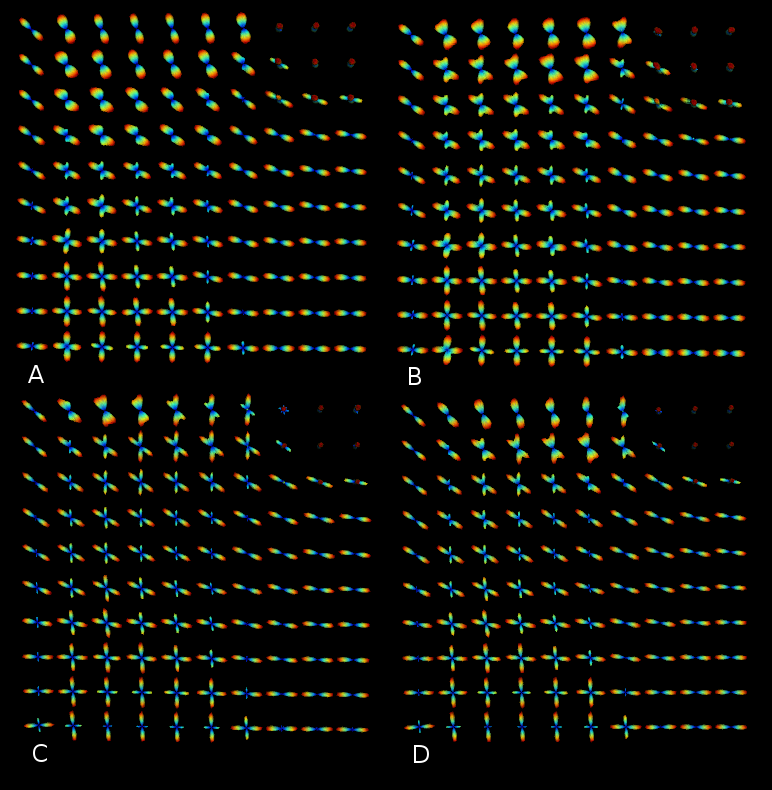
\includegraphics[scale=1.2]{csd_sdt_snr10}
\end{centering}
\caption{ROI [14:24, 22, 23:33] of the denoised test dataset (SNR 10) provided by the organizers of the HARDI reconstruction challenge 2013. A) CSD DTI, B) SDT DTI, 
C) CSD HARDI, D) SDT HARDI.}
\end{figure}

 In order to find the best parameters for the methods described here we created a connectivity matrix after generating deterministic streamlines from the ODFs of the training set. We finally selected the parameters which minimized the number of missing and false bundles in the training set and used those with the test data.
 In Fig.1 we see results from an ROI from slice Y=22 of the testing dataset reconstructed with CSD in A and C and with SDT in B and D. The spherical harmonic order used for the DTI datasests was 6 and for HARDI 8 both for CSD and SDT. In Fig. 1 we observe that SDT performed better in the DTI category but CSD performed slightly better the HARDI category as it managed to resolve more crossing fibers. For the challenge we submitted all results with ODFs saved as spherical harmonic coefficients of order 8. The source code for the methods described in this paper is available at dipy.org.

\bibliographystyle{ieeetr}
\bibliography{/home/eleftherios/Documents/scil-bibtex/scilBibTex}

\end{document}


